\section{Introduzione}
\todo{Da qualche parte bisogna riportare la grammatica da cui si parte (copiare quella che mettiamo nella doc tecnica? Direi di si a grandi linee)}

L'applicazione \textit{ltspice2circuitikz} permette di convertire un file proveniente dal simulatore \textit{LTSpice} (file .asc) in un documento contente il codice latex che rappresenta il circuito simulato tramite l'utilizzo del package \textit{CircuiTikz}. Inoltre, è in grado di mostrare un file pdf che mostra il circuito corrispondente al codice latex generato e, nel caso di errori di formattazione del file in ingresso, è possibile visualizzare un file .asc formattato nel modo corretto. 

\section{Installazione}
L'applicazione è disponibile solo per PC Windows. Per installare l'applicazione è sufficiente decomprimere la cartella compressa \textit{"ltspice2circuitikz app.zip"}. Una volta decompressa, assicurarsi che il contenuto della cartella sia uguale al seguente (figura \ref{fig:contenuto}):

\begin{figure}[h!]
	\centering
	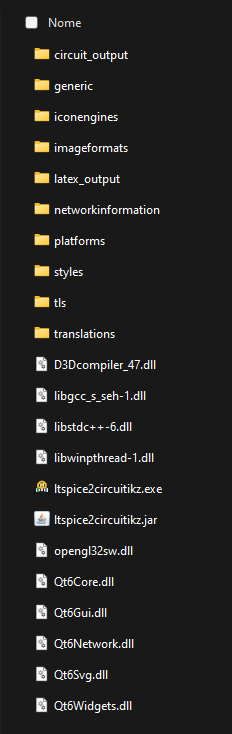
\includegraphics[width=0.25\textwidth]{./ImageFiles/contenuto.png}
	\caption{Contenuto della cartella \textit{"ltspice2circuitikz app.zip"}.}
	\label{fig:contenuto}
\end{figure}

L'applicazione è stata realizzata utilizzando le librerie Qt e l'ambiente di sviluppo Qt IDE. Il componente che si occupa di eseguire la verifica e la traduzione, invece, è stato realizzato in Java. Per il corretto funzionamento dell'applicazione è necessario che sul PC sia installato Java. Per lanciare l'applicazione è sufficiente cliccare due volte sul programma \textit{ltspice2circuitikz.exe}.

\section{Funzionalità}
L'applicazione \textit{ltspice2circuitikz} permette di convertire i circuiti generati con il simulatore LTSpice in documenti latex che utilizzano il package \textit{CircuiTikz} per disegnare il circuito in questione. In figura \ref{fig:schema} sono mostrati i file di input e output dell'applicazione. 
\begin{figure}[h!]
	\centering
	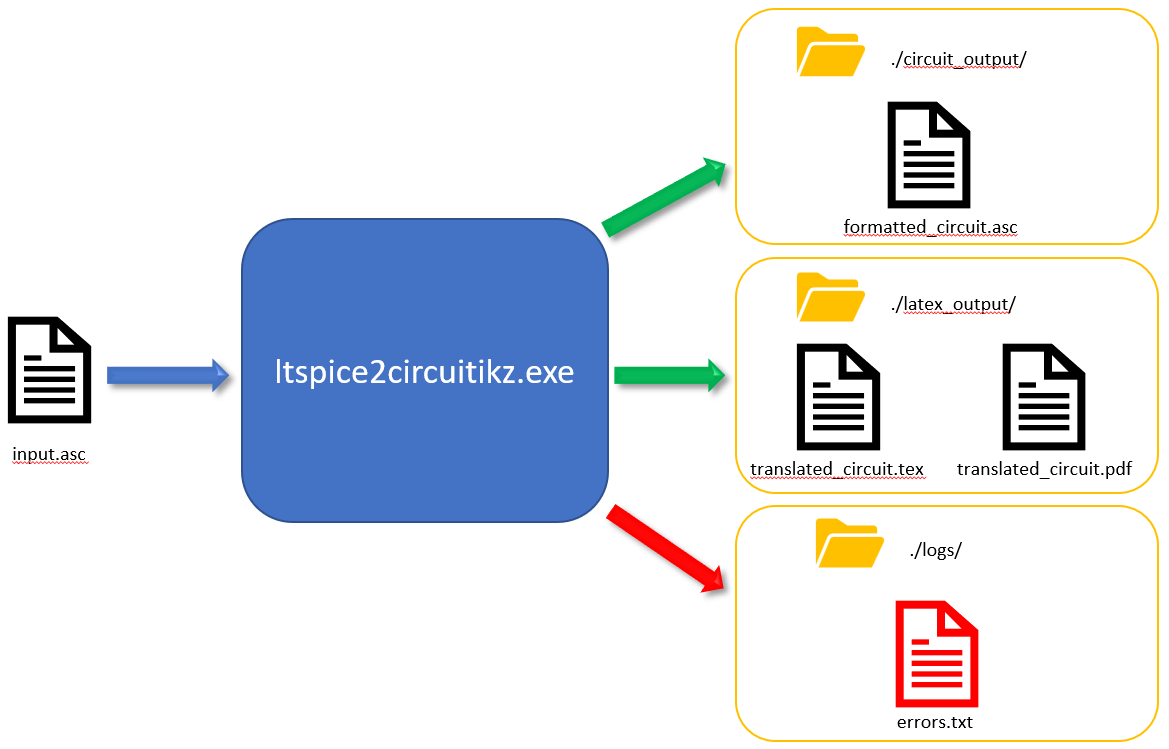
\includegraphics[width=1\textwidth]{./ImageFiles/schema funzionamento.png}
	\caption{File in input e output dall'applicazione.}
	\label{fig:schema}
\end{figure}
Dopo aver generato un file con estensione .asc tramite il simulatore LTSpice, è possibile selezionare tale file per la generazione del circuito in latex. L'applicazione \textit{ltspice2circuitikz} analizza il file in ingresso alla ricerca di errori sintattici e/o semantici. Nel caso in cui non siano presenti errori, viene eseguita la traduzione e vengono generati tre file:
\begin{itemize}
	\item \textit{translated\_circuit.tex}: contiene il testo in latex che utilizza il package \textit{CircuiTikz} per generare il circuito in un documento latex;
	\item \textit{translated\_circuit.pdf}: è il file pdf generato a partire dal file latex che contiene il circuito. È utile per poter verificare che il circuito generato sia corretto;
	\item \textit{formatted\_circuit.tex}: contiene il testo del file .asc formattato in modo corretto.
\end{itemize}
Nel caso in cui, invece, siano presenti degli errori, questi vengono mostrati nella console dell'applicazione. Inoltre, gli errori generati vengono salvati in un file \textit{errors.txt} all'interno della cartella \textit{./logs/}.
Durante la generazione del file latex, vengono tenute in considerazione le dimensioni del circuito che si vuole generare e, nel caso in cui la larghezza superi l'altezza, il circuito generato verrà ruotato automaticamente per sfruttare meglio lo spazio disponibile. 

\clearpage

\section{Esempio di utilizzo}
Di seguito viene mostrato come utilizzare l'applicazione \textit{ltspice2circuitikz}. 

1. Aprire l'applicazione \textit{ltspice2circuitikz} cliccando due volte l'eseguibile \textit{ltspice2circuitikz.exe}. Si aprirà una schermata come quella mostrata in figura \ref{fig:punto_1}.


\begin{figure}[h!]
	\centering
	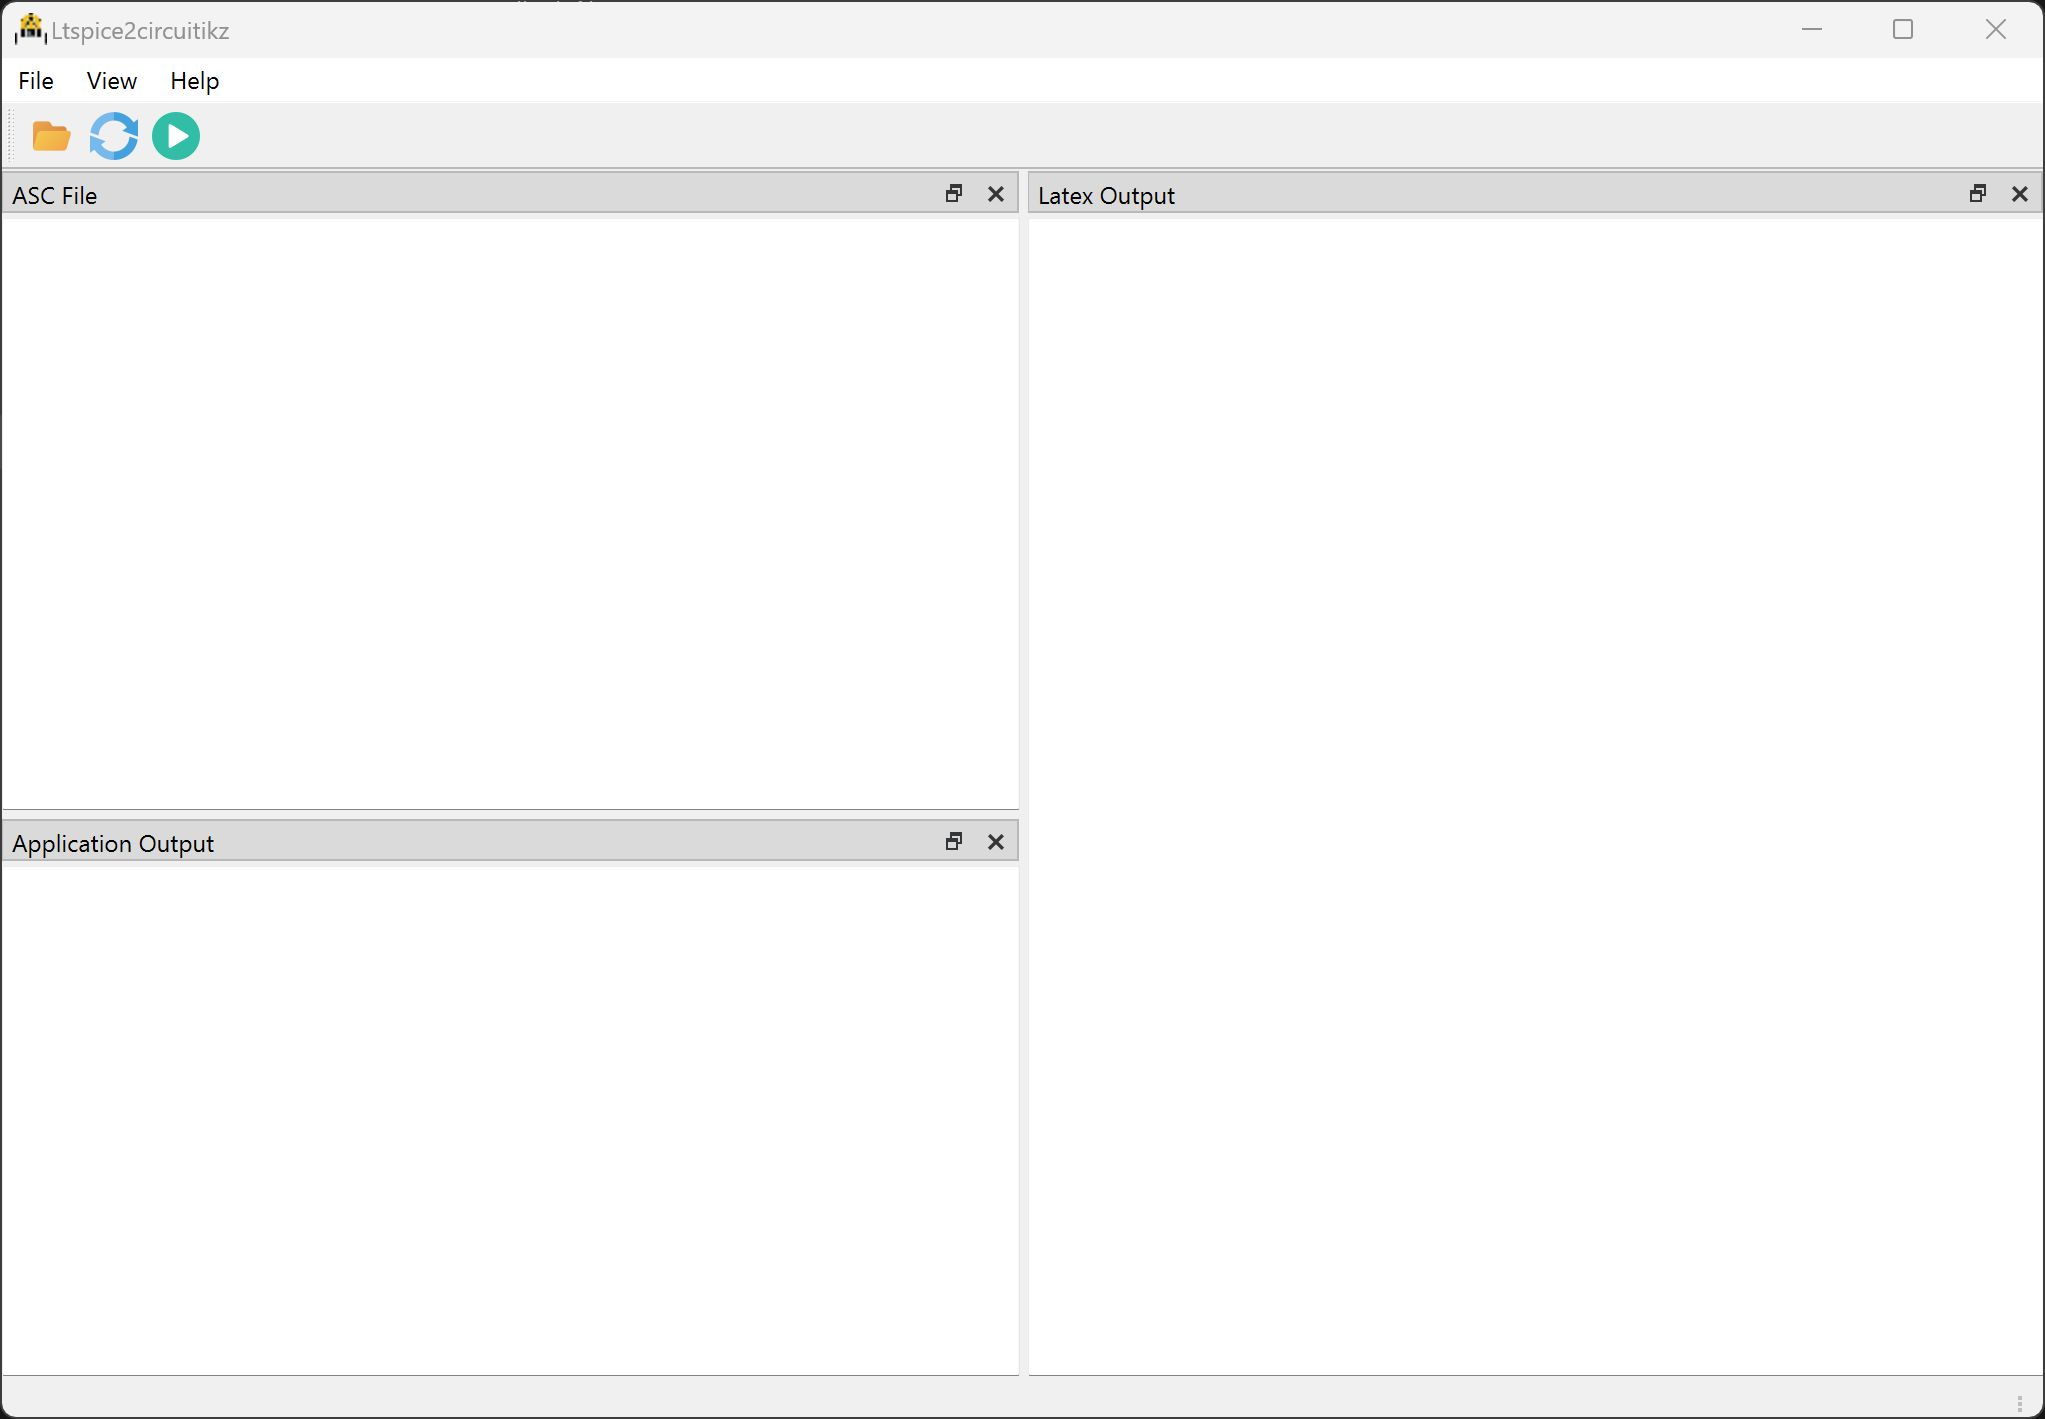
\includegraphics[width=0.7\textwidth]{./ImageFiles/mainview.png}
	\caption{Schermata principale dell'applicazione.}
	\label{fig:punto_1}
\end{figure}

2. Cliccare l'icona \textit{"Open File"} e selezionare un file .asc da aprire. Una volta selezionato il file, il suo contenuto verrà mostrato nella finestra in alto a sinistra (figura \ref{fig:punto_2}). Il contenuto del file non può essere modificato dall'applicazione ma deve essere modificato da un tool esterno. Nel caso venga modificato è possibile ricaricare il file premendo l'icona di \textit{"Refresh"}.
\begin{figure}[h!]
	\centering
	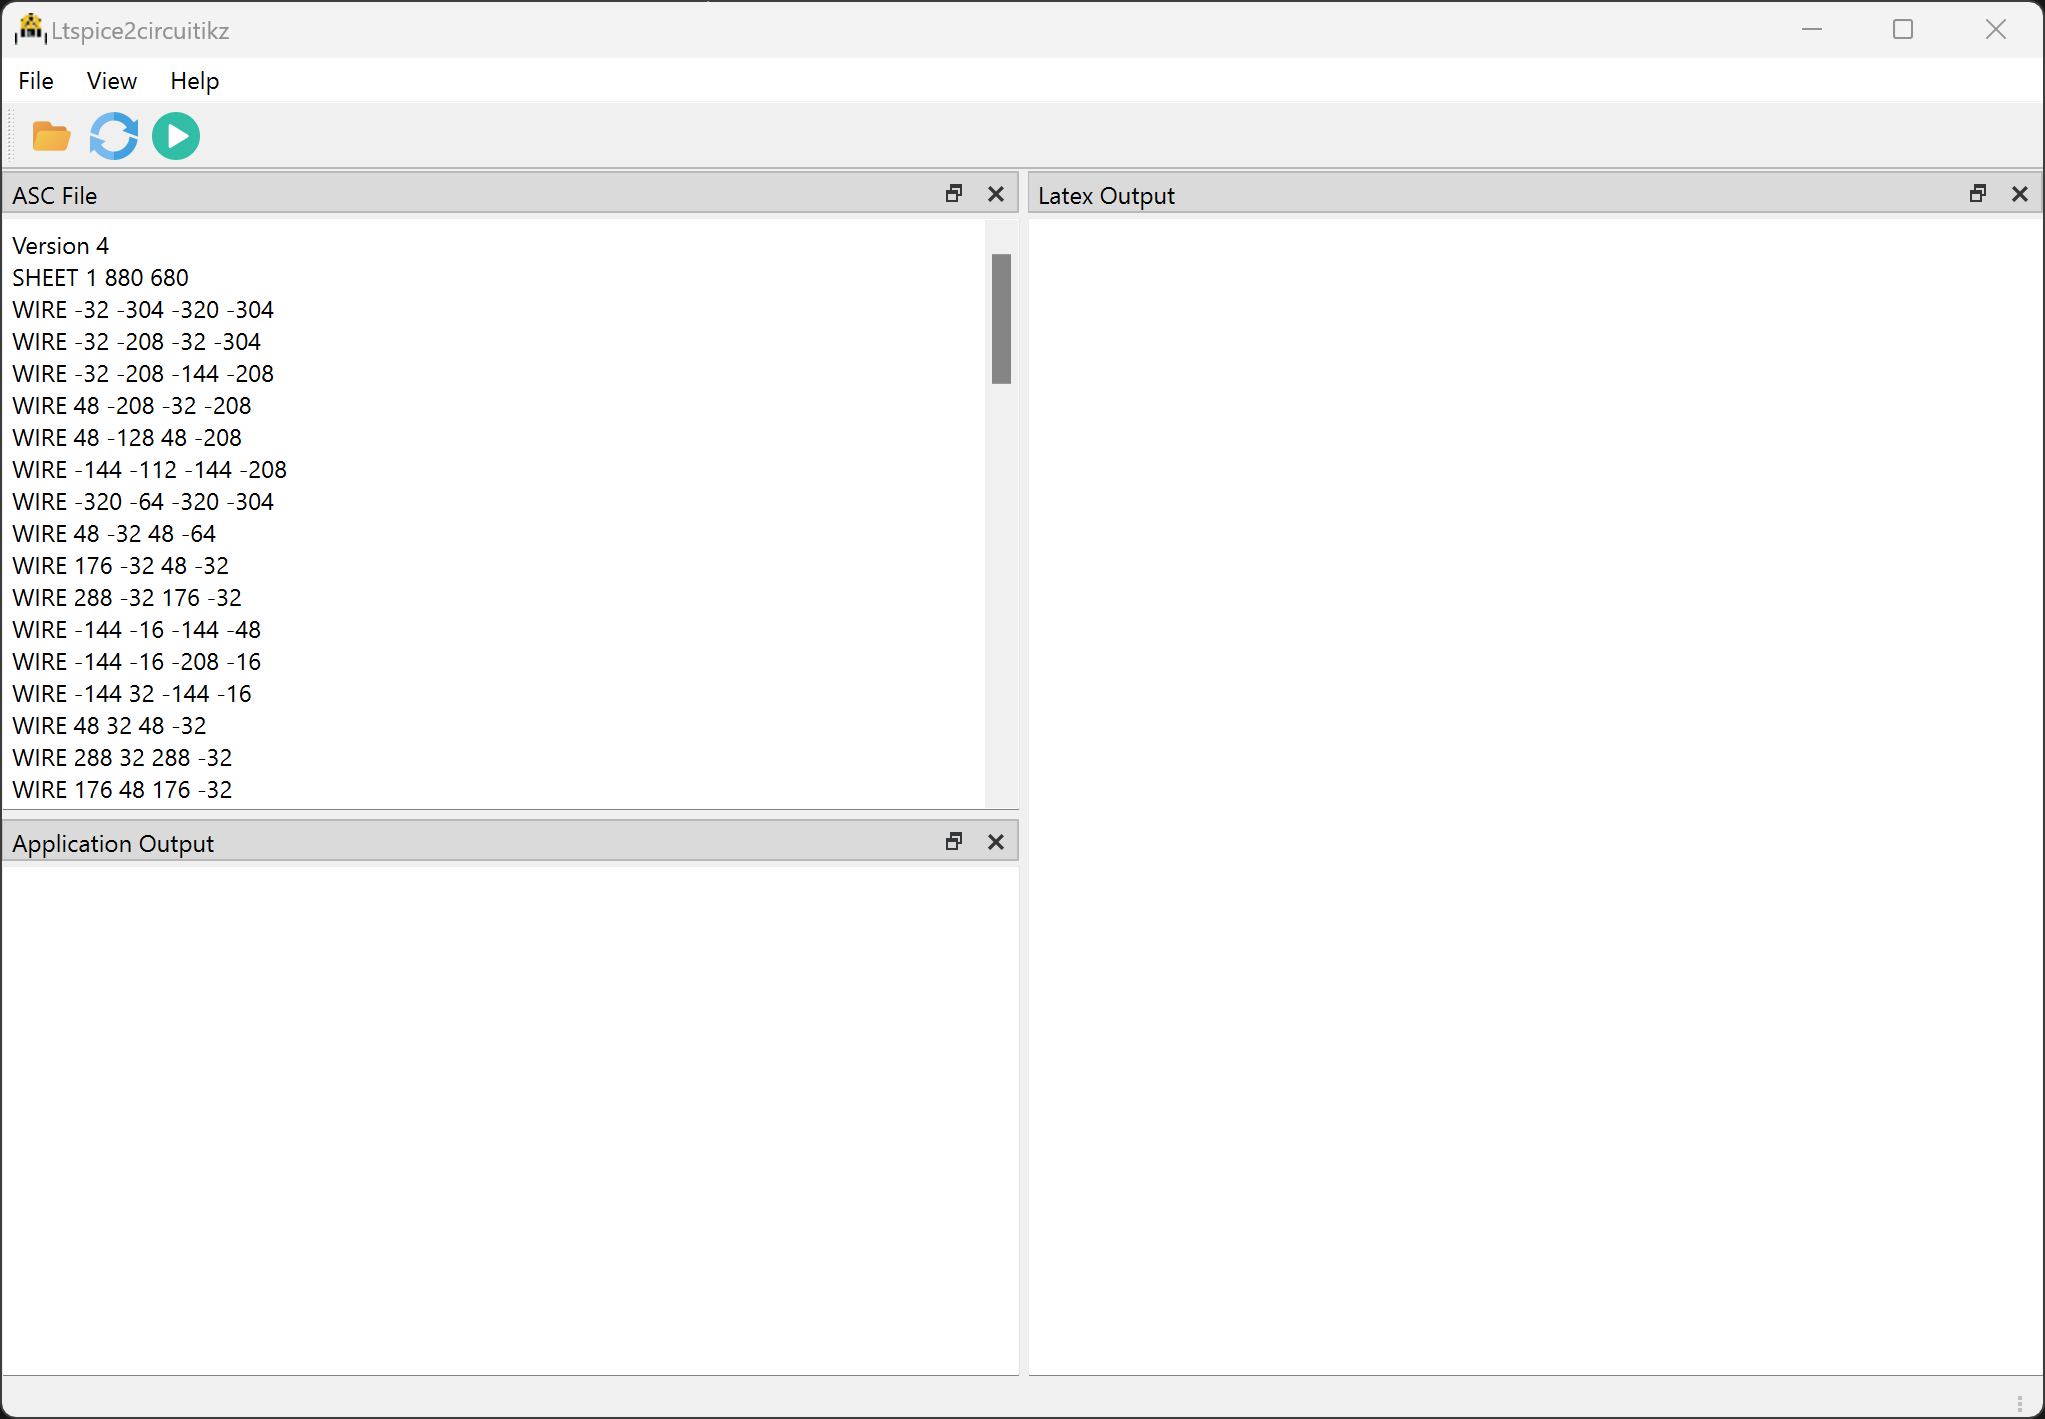
\includegraphics[width=0.7\textwidth]{./ImageFiles/file aperto.png}
	\caption{Schermata che mostra il file aperto.}
	\label{fig:punto_2}
\end{figure}

3. Premere il pulsante verde \textit{"Run"} per lanciare il processo di conversione. Se non ci sono errori, viene mostrato un messaggio verde nell'\textit{Application Output} e viene caricato il contenuto del file latex nella colonna di destra (figura \ref{fig:punto_3}). Inoltre, viene aperto il file pdf contenente il circuito generato. Se si vuole mostrare anche il file formattato in modo corretto, è sufficiente selezionare la voce \textit{"Formatted ASC File"} nel menù \textit{"View"}.
\begin{figure}[h!]
	\centering
	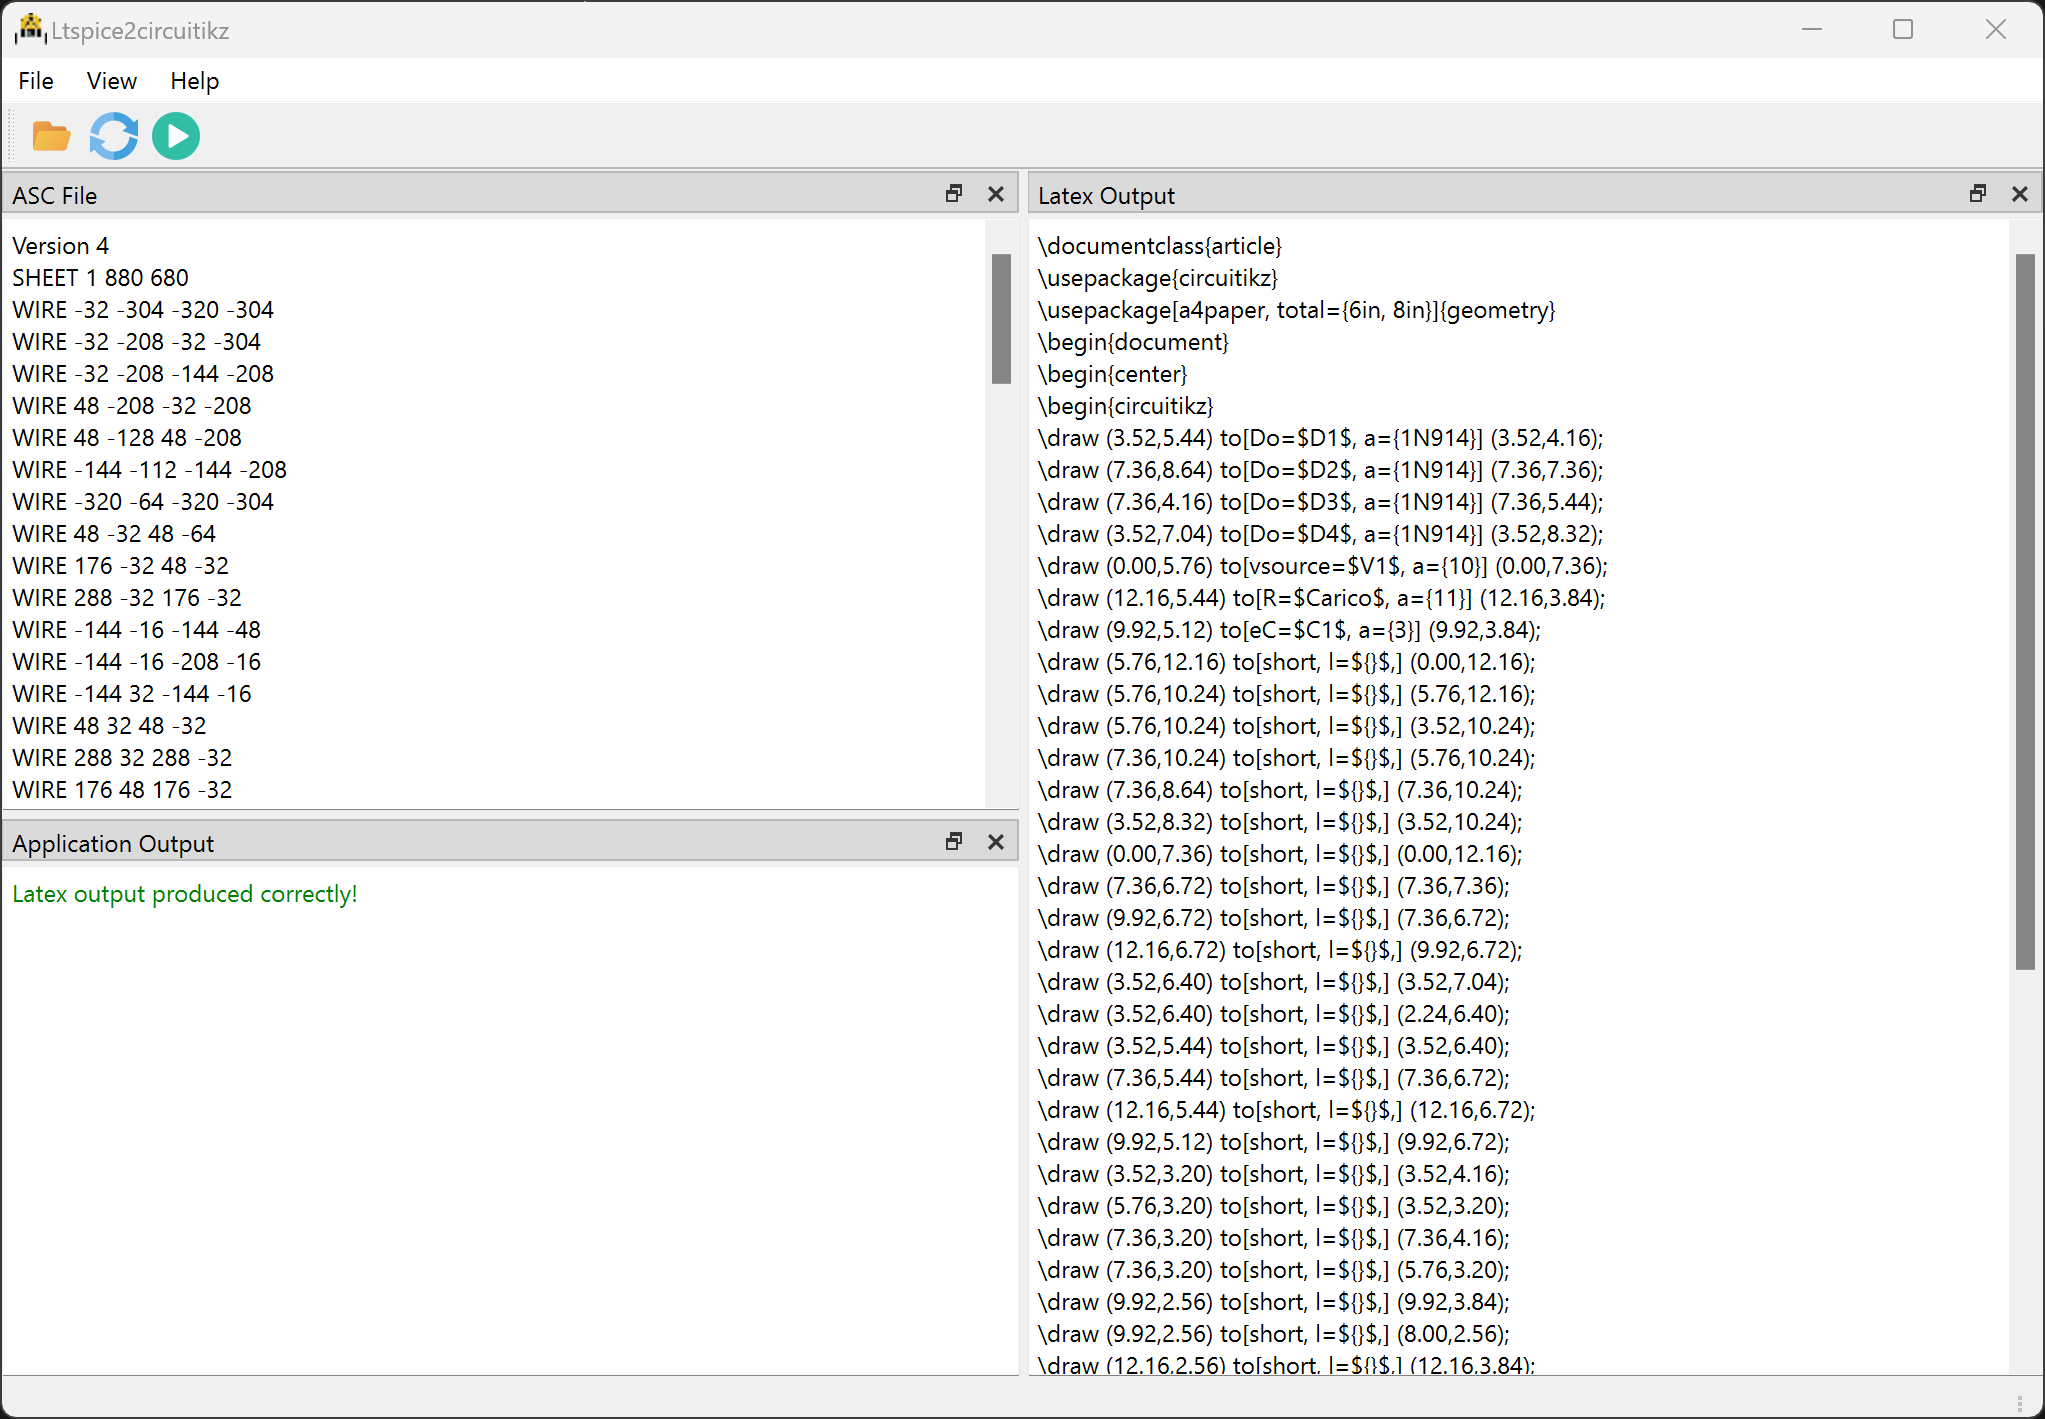
\includegraphics[width=0.7\textwidth]{./ImageFiles/run con successo.png}
	\caption{Processo eseguito con successo.}
	\label{fig:punto_3}
\end{figure}

4. Nel caso in cui ci siano errori semantici o sintattici, il processo si interrompe e nell'\textit{Application Output} vengono mostrati gli errori (figura \ref{fig:punto_4}).

\begin{figure}[h!]
	\centering
	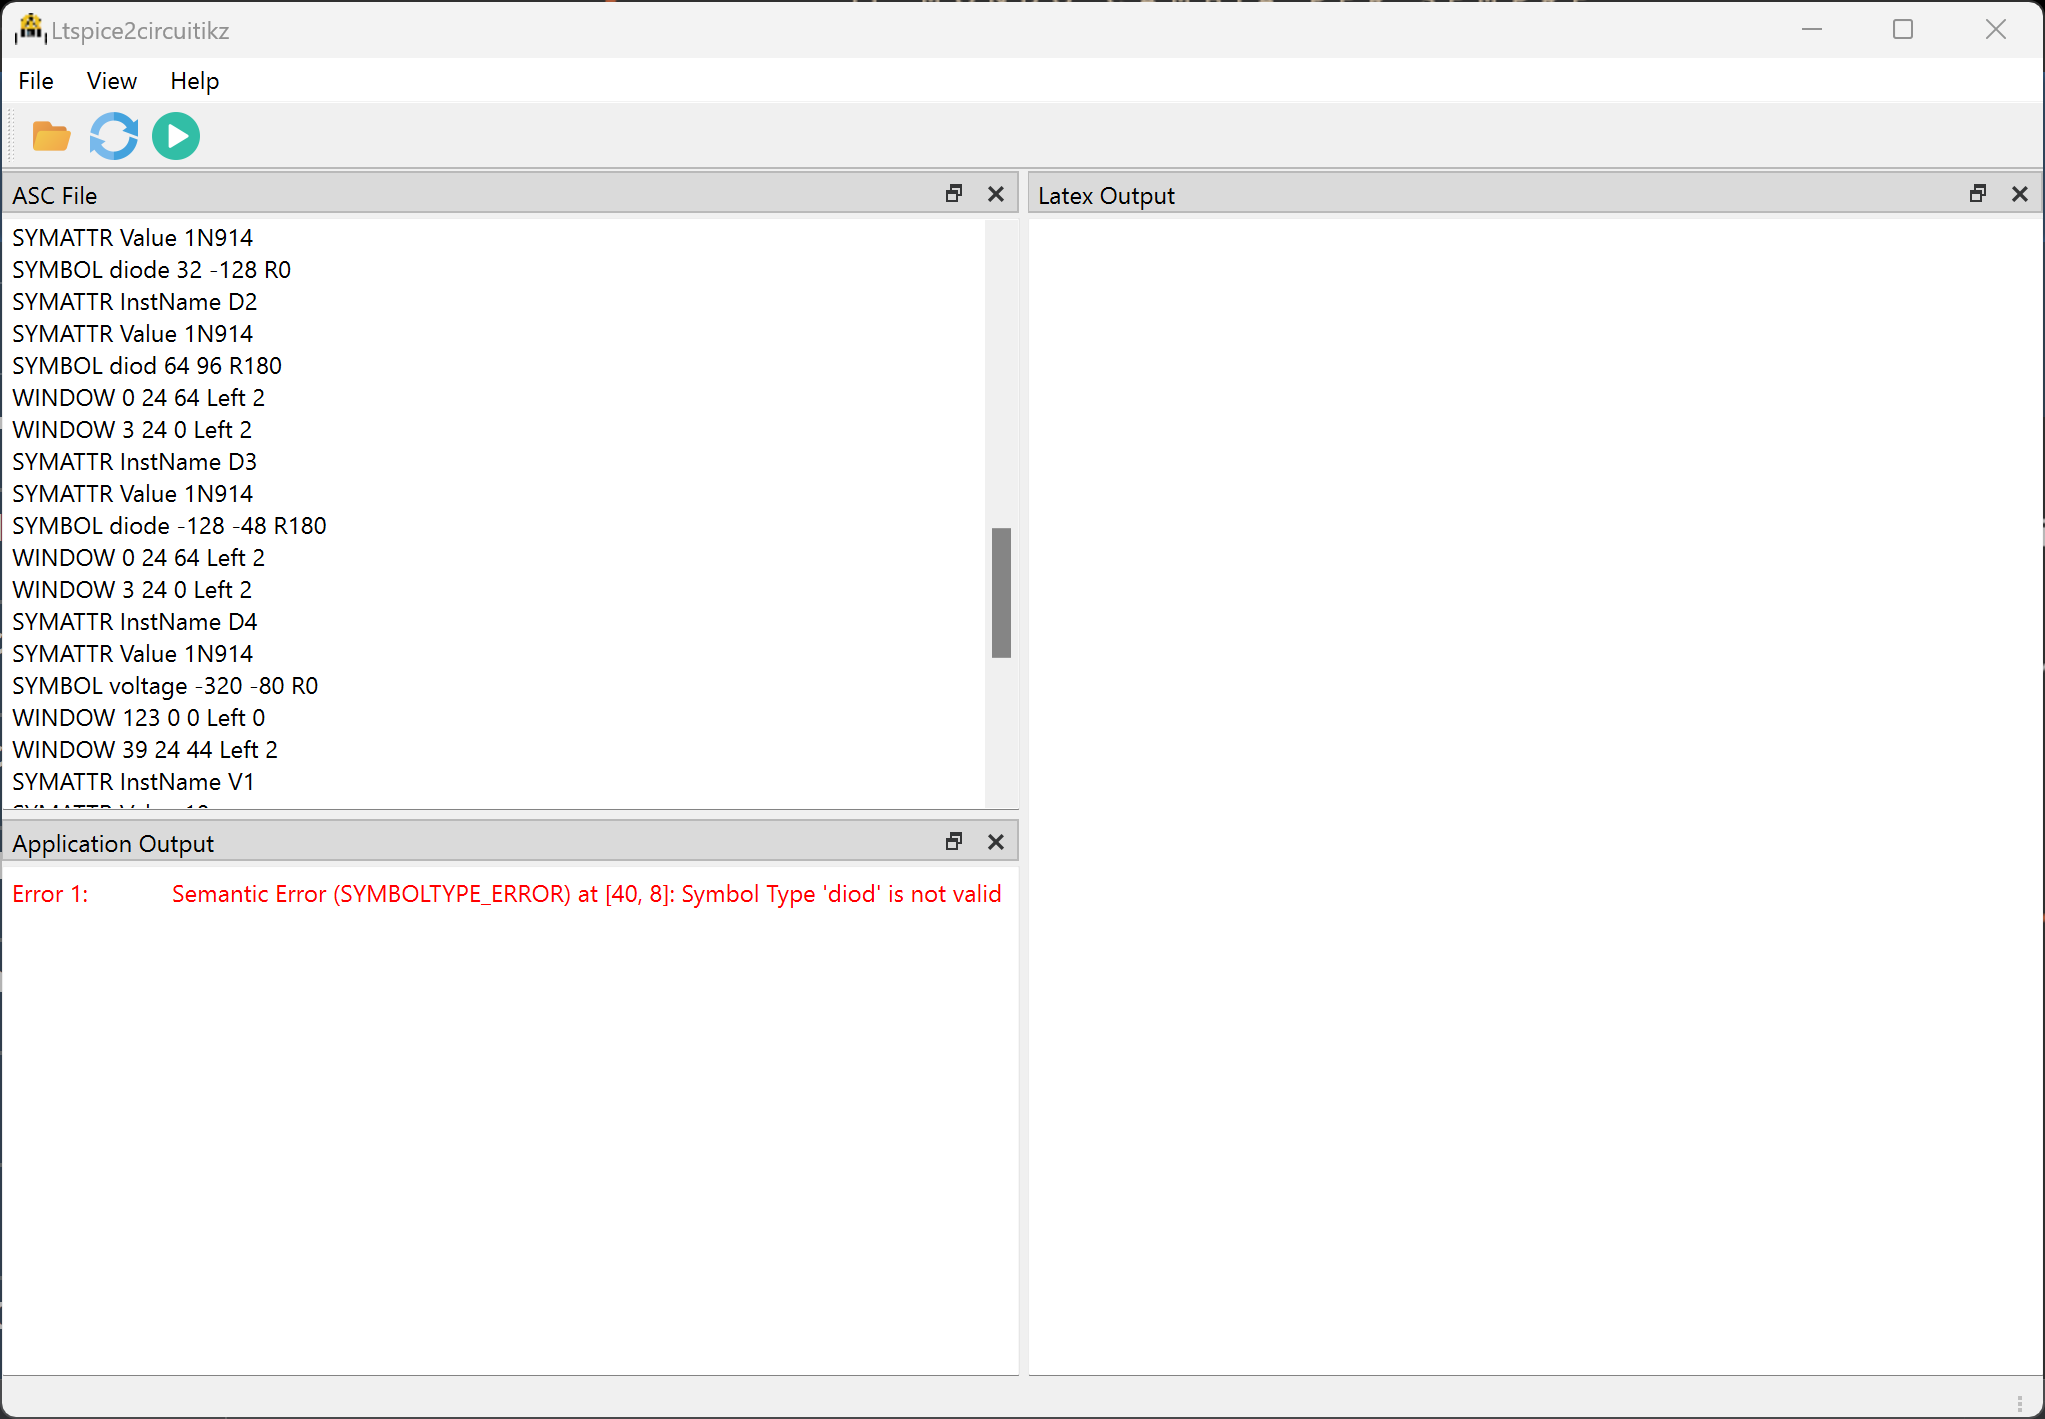
\includegraphics[width=0.7\textwidth]{./ImageFiles/semantic error.png}
	\caption{Processo eseguito con successo.}
	\label{fig:punto_4}
\end{figure}






